\documentclass[12pt]{article}
\usepackage[a4 paper, portrait, margin=1in]{geometry}
\title{EGYPT\\Farmers to Pharoahs}
\author{Derrick Diana\\Harry Heathcock\\Kaedon Jon Williams}
\date{\today}
\usepackage{multicol}
\usepackage{graphicx}
\graphicspath{ {Figures/} }

\begin{document}
	\maketitle
	\begin{abstract}
		Reimplementing a simulation for Ancient Egyptian Farming Communities in Python with a focus on speed and extensibility, from code originally written in Netlogo, with minor changes for cohesion and ease of use as well as quality of life improvements. Testing showed that there were differences between the original simulation and the reimplementation, even when the reimplementation was run in legacy mode.
	\end{abstract}
	
	\section{Introduction}
		Studying ancient civilisations can be difficult due to incomplete information and an inability to test hypotheses. This is a problem which can be partially solved by simulation, if the simulation can be shown to be accurate. A programme was created to reimplement an older simulation model for ancient Egyptyian farming communities in a new language to allow for extensibility and speed improvements, as well as improving the user experience. Another goal was to test whether the model was resilient to slight changes that would be resultant from a reimplementation.\\
		The simulation itself could provide assistance to researchers attempting to study ancient Egypt, allowing them to view how the conditions that were discovered came about in the first place. This could provide insight as to whether slight changes in initial conditions would create a different environment entirely.\\
		The simulation itself is an agent based model, where households claim and farm fields around the Nile River for the grain which they need to survive. Households are each part of a Settlement, which can contain many households. Households grow and thrive, while others die out.\\
		The design process used followed a few steps. The first step was to read and understand the original source code, collecting required functionality and trying to piece together how the system worked as a whole. Once the system was understood, step two began, in which the basic pieces were implemented into an object-oriented python version. This was split into the simulation and the UI, with the simulation very closely following the original code and the UI using the original as a style guide. Once the basics of the simulation and the UI had been created, a set of available data was agreed on and the two systems were brought together. The UI code instantiated a copy of the simulation code, pulled the data required for rendering each year and called the function which causes the simulation to continue for another year. From there, the final step was just to continue programming features into the simulation and UI separately until both fulfilled the original requirements.
	\section{Requirements}
		\subsection{Functional}
			\subsubsection{The simulation should produce graphs to display state}
				This was achieved through the use of FigureCanvasTkAgg() objects as described in the implementation section. This creates a pair graphs which the user can interact with and choose to display any two of the 11 available graphs at any one time.
			\subsubsection{	The user should be able to change inputs to the system}
				This was achieved through tkinter scale widgets and check boxes which are also described in the implementation section. Users can slide the scales to change starting conditions within the limits set in the original code.
			\subsubsection{The simulation should run for a fixed period}
				This is due to the limited applicability of the model, as the simulation is not meant to run for more than 500 years. This was achieved using a counter, that once passed causes the play and step buttons to be greyed out and unusable, forcing the user to click the reset button rather than pushing the simulation beyond its range of applicability.
			\subsubsection{A window should display the area in which the simulation is taking place, displaying the settlement and field positions}
				This was achieved using a tkinter canvas object as described in the implementation section. Logic was written to interpret the state of the simulation and translate that into icons on a grid. The meaning of each of these icons is described in the user manual.
			\subsubsection{The code base should be easily extensible}
		 
		\subsection{Non-Functional}
			\subsubsection{The system should be able to display at least 1 frame per second when running at the highest simulation speed possible}
				This was easily achieved as the program can display at least 5 frames per second even at the highest settings.
			\subsubsection{Code should be structured to allow for easy understanding of functionality and allow functions to be easily swapped out (extensibility)}
				This has been achieved through the majority of functionality which is likely to be changed being placed inside of a single class. This allows for replacing the decision-making of the agent to be replaced simply by replacing a few functions of a single class, which have documented functionality as described in the technical API manual.
			\subsubsection{Inputs should be controlled by sliders for each of the initial conditions}
				This has been achieved through the use of Tkinter Scale widgets to provide input to the program.
			\subsubsection{The interface should be user friendly and easy to use}
				This has been achieved through displaying a tooltip which describes what each widget on the screen does when the mouse hovers over it as described in the implementation section.	
			
		\subsection{Usability}
			The following factors were considered when designing the user interface:
			\subsubsection{Error prevention}
				In order to prevent errors from occurring, buttons which cannot be clicked at any time are disabled. In addition, since sliders cannot be changed while the program is running they too are disabled (indicated by being greyed out) until the reset button is clicked. 
			\subsubsection{Performance}
				All of the following statements refer to the program being run on a modern CPU. With the display on, the program runs 1000 years in about 45 seconds if the graph rate is set to its default value of 30. If this value is changed to 100, the time taken to run drops to 25 seconds. If the user only wants the final results of the simulation, the simulation may be run without updating the display. In this case, the program runs about 1000 years in 15 seconds. 
			\subsubsection{Learnability}
				In order to ensure learnability, a tool tip is constantly displayed on the bottom of the interface to ensure that the user is able to have a live description of what each component does. In addition, a user manual was created and included in this document.
			
		\subsection{Use Cases}
			\subsubsection{As an Archaeologist/ general user wanting to run the simulation}
				I want to be able to change input parameters before running the program to see how the results of the program are affected.\\
				\textit{Resolution:} To do this, the user may select and drag any of the sliders on the left before the simulation has started running, and on doing so the simulation will reset the simulation with the changed inputs.
			\subsubsection{As an Archaeologist/ general user wishing to analyse results}
				I want to save one or more of the displayed graphs for later analysis.\\ \textit{Resolution:} To do this, the user may either save individual figures by clicking the save icon under the figure or clicking the Save All Figures button.
			\subsubsection{As an Archaeologist/ general interested experimentalist}
				I want to be able to run a large number of simulations, analyse and compare the data from different runs.\\
				\textit{Resolution:} the inclusion of a Run Multiple button which allows the user to run the entire simulation as many times as the user wishes and the output graphs from each run are each saved in their own folder, within a larger containing outer folder.
			\subsubsection{As an Archaeologist/ general interested experimentalist}
				I want to be able to view details about the internal state of the system at any time in order to see how parameters change from one year to the next.\\
				\textit{Resolution:} the user may pause the simulation and then right click on any block that they wish to see the parameters of. This will cause a pop-up to appear next to the block displaying information about the block.
			\subsubsection{As an Archaeologist/ researcher wishing to present findings to others} 
				I want to be able to be able to repeat runs and have the exact same starting set up in order to be able to reproduce results to show others and reduce the number of uncontrolled variables in experiments.\\
				\textit{Resolution:} The user is able to click the text-box "manual-seed-enabled" which allows them to enter a 'seed' which is a specific string of characters. So long as the user enters the same string the next time, the starting positions of the settlements will be identical. 
		
	\section{Design Overview}
		The programme was designed such that the only interactions between the simulation itself and the UI are in instantiation, the increase of years and the current state of the simulation. This was done for encapsulation purposes and to ensure the integrity of the simulation at all times. The display is split up into the UI and the rendering of the simulation, this was performed for ease of upkeep, as combining the two would result in a monolithic structure which is difficult to work with and maintain. The basic structure is shown in Figure \ref{fig:Architecture}.\\
		Due to this being a reimplementation of work that has already been done, the algorithms and data structures were pre-determined. All changes made to the overall algorithm were due to efficiency concerns, or strange behaviour which was corrected.\\
		Data was stored almost exclusively in lists, as order needed to be randomised each tick to remove possible biases due to ordering of operations being performed on the households.\\
		
		\begin{figure}[!htb]
		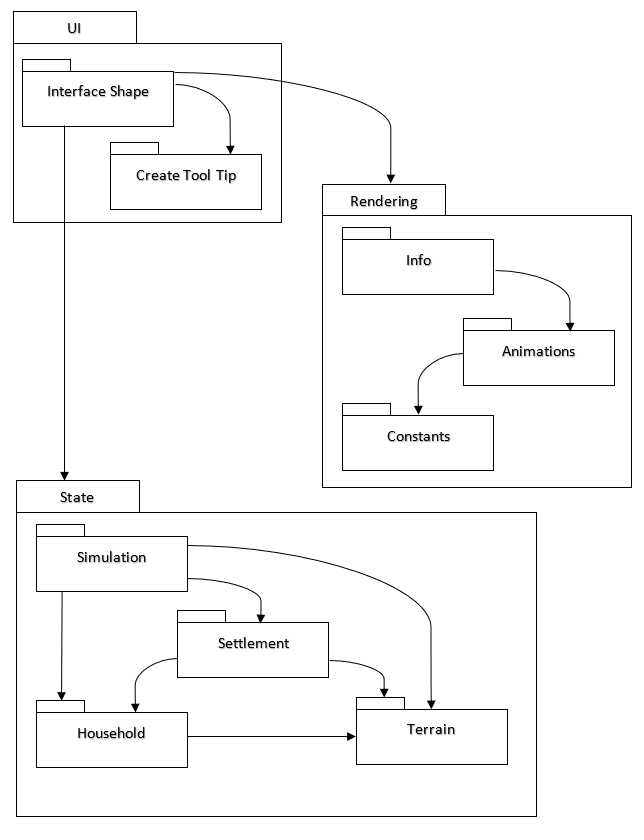
\includegraphics[width=10cm]{ArchitectureDiagram}
		\caption{Architecture diagram for the system, showing how the UI checks the state of the simulation and passes this to be rendered.}
		\label{fig:Architecture}
		\end{figure}
	
		\subsection{Changes}
			A number of changes in the implementation were made, some due to what seemed to be implementation errors in the original code and others due to functionality not making sense with what was trying to be achieved. Those which affect functionality have been implemented as explained, however when the Legacy Mode setting is enabled, these changes are reverted back to how they were in the original implementation.
				\subsubsection{Death Due to Lack of Grain}
				In the original NetLogo code, if a household did not have enough grain to survive a year then a single person would die and the grain would be set to zero. In reality this doesn't make sense, as if a household has no food, then no one would survive. The reimplementation changed this so that only the family members who can be fed will survive.\\
				\subsubsection{Population Increases}
				In the original code, if the total current population is less than or equal to the historical projected population then the population can increase. At first glance this seems to be correct, however this allows the population to always grow slightly faster than the projected historical value, and thus in the reimplementation this is changed so that the population will only increase if it is less than the historical projected population.\\
				\subsubsection{Generational Changes in Ambition and Competency}
				In the original code, if the ambition or competency for a household moved out of the bounds set (minimum, up to 1) then a new value would be generated until it fell within the bounds. This means that the computational time for the ambition and competency changes are unbounded. In the reimplementation, a value within the possible range is generated.\\
				\subsubsection{Order of Field Claimants}
				In the original code, households claimed fields in ascending order of how much grain they currently have. This seemed inconsistent with every other operation being independent of grain or ordering, in the reimplementation, this ordering is randomised each year.
	\section{Implementation}
		As can be seen in Figure \ref{fig:Packages}, InterfaceShape is the controller class which invokes other methods in all other classes. InterfaceShape contains the code which sets up the GUI, which consists of the components explained below.\\		
		A canvas object on which the main simulation grid is drawn. The main simulation grid displays the households, fields and rivers distinctly and clearly. A panel, that consists of slider and check-box objects, which allows the user to initialise parameters for the simulation. Two FigureCanvasTkAgg() objects which act as widgets and each create a matplotlib-style interactive graph. These graphs can be zoomed, scrolled, and can save their displays as images. These are live representations of figure objects within the matplotlib.pyplot library. Several other buttons and sliders which allow the user to interact with the program in minor ways.\\
		
		\begin{figure}[!htb]
			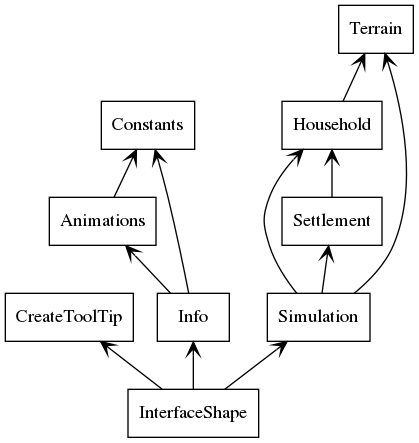
\includegraphics[width=10cm]{packages}
			\caption{Diagram showing the relationship between all the classes involved in the programme.}
			\label{fig:Packages}
		\end{figure}
		
		\subsection{Important Functions in the GUI and Rendering}
			The GUI has a method called MainLoop, which performs the primary actions corresponding to one year of the simulation which includes calling the following methods, in order:
			\begin{itemize}
				\item Simulation.tick()\\
				Which causes the simulation class to simulate a single year, generating and setting fertility values for the entire set of land, allowing households to claim, farm and rent land, as well as consuming grain, dying out when not enough food is present, allowing for population growth as well as shifts in the household competency and ambition levels.
				\item Info.drawGridSimulation()\\
				Which accesses the simulation object, finding the positions and values for fields and settlements in order to render them on the canvas correctly.
				\item Info.plotData()\\
				Which reads the necessary data out of the simulation object and appends all the data needed for each graph to a list which stores the lists required for each graph. This outer list consists of 11 inner list, each corresponding to a single graph.
				\item Info.updateGraphs()\\
				Which takes the data which has already been stored and adds it to the pyplot.figure objects which the FigureCanvasTkAgg() objects represent. In order to reduce the time taken to draw all the points, only points which have been added since the last draw are drawn each cycle. This is performed until the user decides to change which graph is being displayed, in which case the entire graph must be redrawn, or many lines have already been drawn, in which case the graph is redrawn as a single line. The second part is a speed optimisation, as plotting many points at once is a slow process, however the fragmentation that is created when many smaller lines have been drawn can cause the process to slow even further.
				\item Info.showGraphs()\\
				Which calls show on both of the FigureCanvasTkAgg() objects to show the data to the user.
			\end{itemize}
			
			The MainLoop method then calls itself again in a non-recursive manner using the tkinter method after(), which calls the MainLoop function again without blocking after a given delay in milliseconds. This number of milliseconds for the delay is determined by a slider that is present in the GUI and the delay is calculated each frame to achieve the desired frames per second. If the desired framerate cannot be achieved, then the programme does not sleep.
		
		\subsection{Important Functions in the Simulation}
			\subsubsection{Simulation}
				The most important function of simulation is tick(). This calls all other functions which are required for the simulation to run for a single year, incrementing all values which need to be incremented. This begins by calling flood(), which sets fertility values in the land. The settlement tick is then called, which is described below, followed by the rentLand() function. The rentLand() function sorts all the households by ambition and allows ambitious households to farm extra land which they don't own. The settlement tock function is then called, also described below.
				
			\subsubsection{Settlement}
				The two most important functions of the settlement are tick() and tock(). The first consists of functions which should be called before land rental can occur, while the latter consists of the functions which should be called afterwards. The tick() function causes each household within the settlement to claim land, and then farm their claimed land. The tock() function causes each household within the settlement to consume grain for the year, and then allows for a change in ambition and competency, as well as allowing for population growth if other values are also met.\\
				
			\subsubsection{Household}
				All of the functions in the Household class are important for the functioning of the simulation, as these are where the individual actions are controlled. The farm() function causes the household to farm its fields, the claimLand() function causes the household to make an attempt at claiming fields in the nearby area, grainTick() consuming grain for the year, populationIncrease() giving the possibility of increasing the population and generationalChange() allows the competency and ambition of the household to change over time.
			
			\subsubsection{Terrain}
				The important functions in the Terrain class are the setFertility(), claim() and unclaim() functions. These are all self-explanatory from the names.
	
	\section{Test Cases}
		To validate the correctness of our simulation we ran it using a variety of different initial conditions and then compared the graphs produced to those of the original simulation. The multiple run feature was used extensively to significantly shorten time spent gathering data. The test cases were all run with legacy mode enabled and so included the bugs of the original. Test initial conditions are set to the defaults unless otherwise specified. The following values constitute the defaults:\\
		\begin{itemize}
			\itemsep-0.5em 
			\item Model time span - 500
			\item Starting settlements - 14
			\item Starting households - 7
			\item Starting household size  - 5
			\item Starting grain - 3000
			\item Min ambition - 0.1
			\item Min competency - 0.5
			\item Generational variation - 0.9
			\item Knowledge radius - 20
			\item Distance cost - 10
			\item Fallow limit - 4
			\item Population growth rate - 0.1
			\item Min fission chance - 0.7
			\item Household fission - disabled
			\item Land rental rate - 50
			\item Land rental - disabled
		\end{itemize}
		
		The households are divided up into brackets based on their current grain amount in comparison to the household with the most grain. The brackets are $>66\%$, $33\%$ to $66\%$ and $<33\%$.
	
		\subsection{Test cases considered}
			\subsection{All values are left at the default}
				\begin{figure}[!htb]
					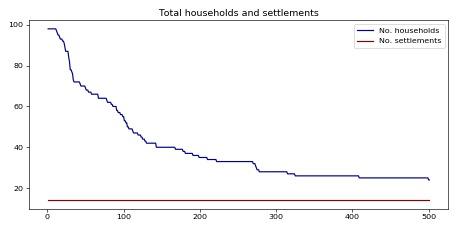
\includegraphics[width=12cm]{Default_values_run1_A}\\
					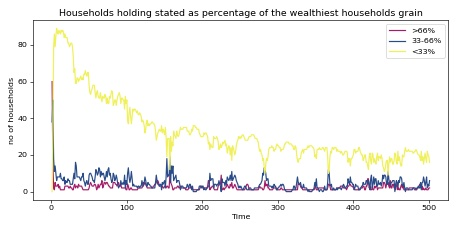
\includegraphics[width=12cm]{Default_values_run1_B}
					\caption{Graphs generated when running the Python reimplementation with default values}
					\label{fig:Default_values_Ours_1}
				\end{figure}
				
				\begin{figure}[!htb]
					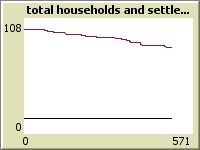
\includegraphics[width=6cm]{Default_values_run1_C}\\
					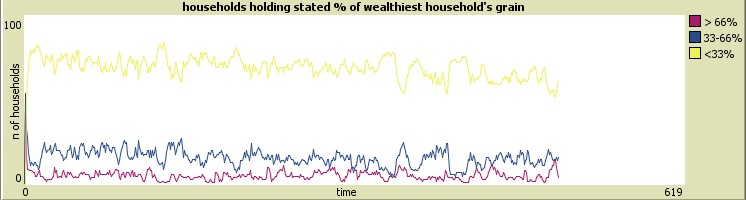
\includegraphics[width=15cm]{Default_values_run1_D}
					\caption{Graphs generated when running the NetLogo implementation with default values}
					\label{fig:Default_values_Netlogo_1}
				\end{figure}
				
				This test was chosen to give a baseline set of graphs to compare all subsequent ones to to give an indication as to whether the desired functionality was achieved, relatively speaking. These will also be compared to ones taken from the original simulation to ascertain correctness.
			
				Expected behaviour is for the households in the upper bracket to be the fewest, the middle brackets the second most and the lower bracket the least. Few settlements should have all their population reduced to 0, if any. 
		
			\subsection{Land rental enabled}
					\begin{figure}[!htb]
					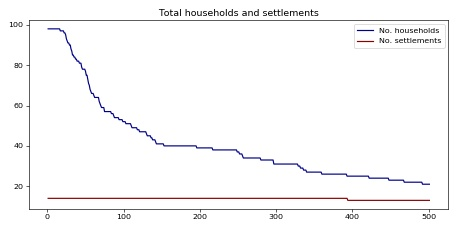
\includegraphics[width=12cm]{Land_rental_enabled_run1_A}\\
					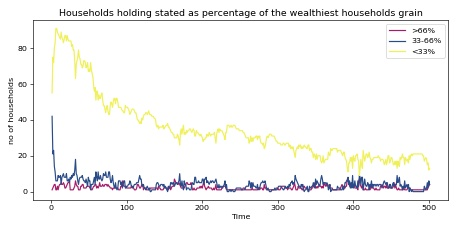
\includegraphics[width=12cm]{Land_rental_enabled_run1_B}
					\caption{Graphs generated when running the python reimplementation with rent enabled}
					\label{fig:Land_rental_enabled_ours_1}
					\end{figure}
					
					\begin{figure}[!htb]
						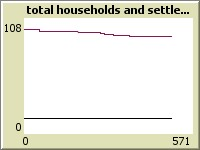
\includegraphics[width=6cm]{Land_rental_enabled_run1_C}\\
						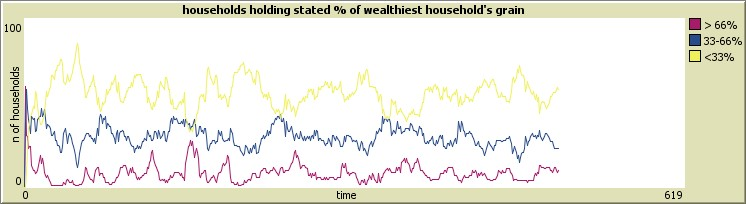
\includegraphics[width=15cm]{Land_rental_enabled_run1_D}
						\caption{Graphs generated when running the NetLogo implementation with rent enabled}
						\label{fig:Land_rental_enabled_Netlogo_1}
					\end{figure}
				This test was chosen to validate the implementation of land rental. The graphs generated shall be compared with the baseline graphs to see if they show the expected differences.
		
				As households descend into poverty and lose fertile fields, they will start to borrow from their neighbours and so bring themselves back from the bad situation they were in, and so fluctuating between poverty and the middle bracket.
		
				The number of households in the lower and middle brackets should fluctuate greatly throughout the simulation, but the number of households in the lower bracket will remain the majority and next will be the households in the middle bracket, though these numbers will be much closer than in the baseline test. 
		
		
			\subsection{Min ambition set to 1}
				\begin{figure}[!htb]
					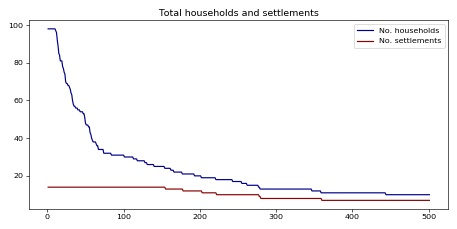
\includegraphics[width=12cm]{Min_ambition_run1_A}\\
					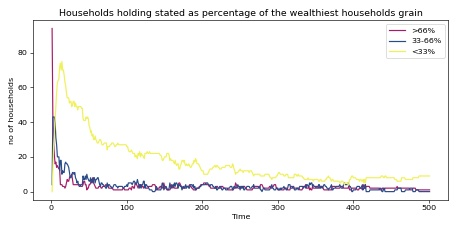
\includegraphics[width=12cm]{Min_ambition_run1_B}
					\caption{Graphs generated when running the python reimplementation with the minimum ambition set to 1}
					\label{fig:Min_Ambition_enabled_ours_1}
				\end{figure}
					
				\begin{figure}[!htb]
					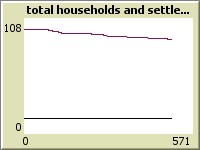
\includegraphics[width=6cm]{Min_ambition_run1_C}\\
					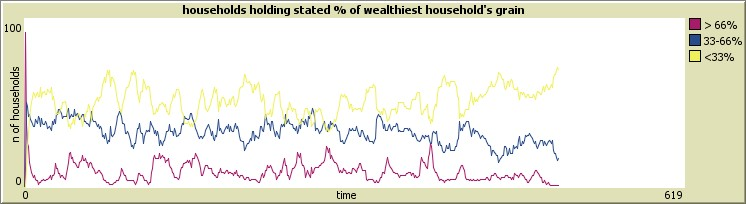
\includegraphics[width=15cm]{Min_ambition_run1_D}
					\caption{Graphs generated when running the NetLogo implementation with the minimum ambition set to 1}
					\label{fig:Min_Ambition_enabled_Netlogo_1}
				\end{figure}
				This test was chosen to validate the implementation of ambition. The graphs generated shall be compared with the baseline graphs to see if they show the expected differences, as well as with the competency graphs to see if they show similar results.
		
				Since everyone is ambitious, everyone will attempt to farm more and so fewer households will become poor and die out.
		
				The majority of households shall be within the middle bracket, next the lower bracket and then the higher bracket. Though, at times, the lower bracket may overtake the middle bracket or be less than the higher bracket.
		
		
			\subsection{Min competency set to 1}
				\begin{figure}[!htb]
				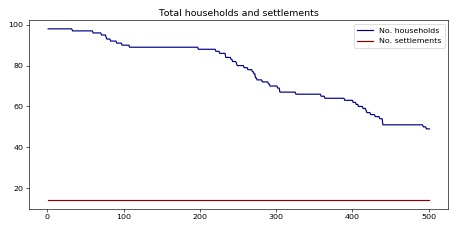
\includegraphics[width=12cm]{Min_competency_run1_A}\\
				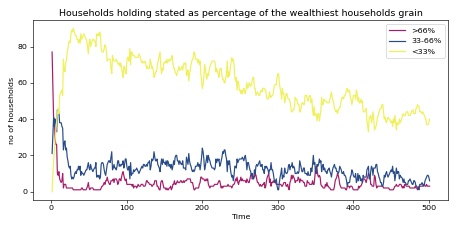
\includegraphics[width=12cm]{Min_competency_run1_B}
				\caption{Graphs generated when running the python reimplementation with the minimum competency set to 1}
				\label{fig:Min_competency_ours_1}
				\end{figure}
				
				\begin{figure}[!htb]
					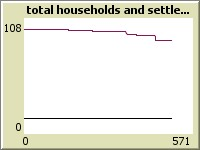
\includegraphics[width=6cm]{Min_competency_run1_C}\\
					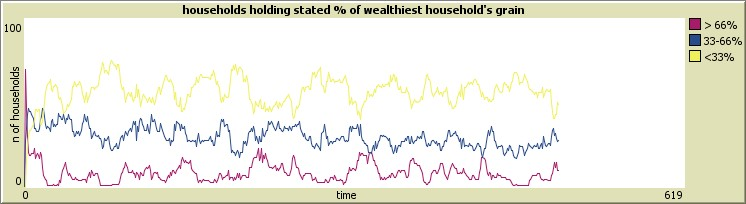
\includegraphics[width=15cm]{Min_competency_run1_D}
					\caption{Graphs generated when running the NetLogo implementation with the minimum competency set to 1}
					\label{fig:Min_competency_Netlogo_1}
				\end{figure}	

				This test was chosen to validate the implementation of ambition. The graphs generated shall be compared with the baseline graphs to see if they show the expected differences, as well as with the ambition graphs to see if they show similar results.
		
				Since everyone is competent, full value is gotten from each harvest and so it should be difficult for any one household to become too poor and die out.
		
				The majority of households shall be within the middle bracket, next the lower bracket and then the higher bracket. Though, at times, the lower bracket may overtake the middle bracket or be less than the higher bracket.
		
		
		
			\subsection{Min ambition and competency set to 0}
				\begin{figure}[!htb]
				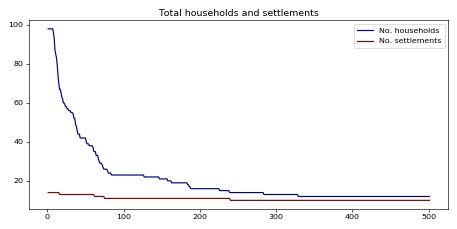
\includegraphics[width=12cm]{Min_ambition_competency_run1_A}\\
				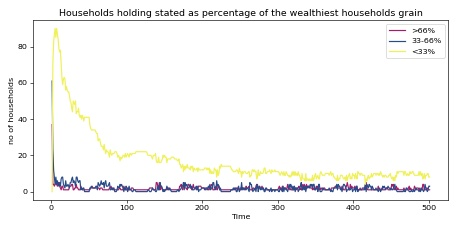
\includegraphics[width=12cm]{Min_ambition_competency_run1_B}
				\caption{Graphs generated when running the python reimplementation with the minimum competency and minimum ambition set to 0}
				\label{fig:Min_ambition_competency_ours_1}
				\end{figure}
				
				\begin{figure}[!htb]
					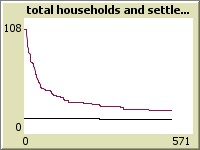
\includegraphics[width=6cm]{Min_ambition_competency_run1_C}\\
					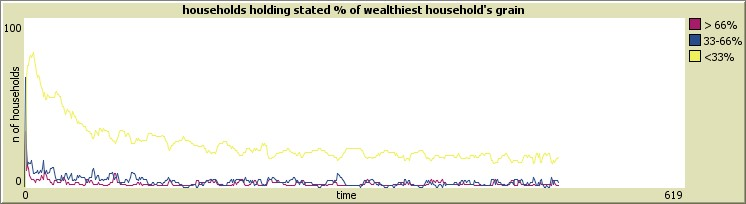
\includegraphics[width=15cm]{Min_ambition_competency_run1_D}
					\caption{Graphs generated when running the NetLogo implementation with the minimum competency and minimum ambition set to 0}
					\label{fig:Min_ambition_competency_Netlogo_1}
				\end{figure}
				This test was chosen to test the other extreme of min ambition and competency. The graphs generated shall be compared with the baseline graphs to see if they show the expected differences.
				
				Households will vary greatly and so there should be a large difference in equality. Since the average household won’t be able to farm particularly well and won’t do so incredibly often, grain values will be low and a lot of households will die out.
				
				The distribution of households between the brackets should be comparable to that of the baseline test, though at lower values of households in each. The gini index will be relatively high and total grain values will be lower in comparison.
		
			\subsection{Household fission enabled}
				This test was chosen to validate the implementation of land rental. The graphs generated shall be compared with the baseline graphs to see if they show the expected differences.
			
				Since households have a chance to split when they grow large, there will be fewer large households and so fewer households in the higher and middle brackets (since they won’t be able to farm as much grain if their workers keep splitting off). 
			
				The difference between the graphs of baseline test and this one will not be that different, however, since fission only comes into effect later on in the simulation (since households don’t grow to enough workers to split particularly quickly), and so does not have time to greatly affect the bracket distribution. The one graph that is affected is the number of households and settlements graph, in which the number of households begins to increase towards the end of the simulation.
		\section{Discussion of Results}
		
			\subsection{All values are left at the default}
				As can be seen, the graphs look quite different. As shown in Figure \ref{fig:Default_values_Ours_1} the household numbers drop off very quickly, which does not correctly represent the original NetLogo simulation (Figure \ref{fig:Default_values_Netlogo_1}). The cause of this problem is not known, but possible theories include the claim land functionality stopping certain household from claiming enough fields to sustain themselves, as well as there being an error in the harvest calculation. 
				While the “Households holding stated percentage of wealthiest household’s grain” graphs do look quite different, they do show the same behaviour of how inequality is distributed between the households when taking into account the error with our households dying off.
		
				So overall a good representation of how inequality is distributed, but not a good representation of how households grow and die off.
		
			\subsection{Land rental enabled}
				Interestingly enough, with rent enabled in our simulation it performs the same or possibly worse than our baseline test. Which is due to negative values being harvested a good amount of the time, which impacts the grain of the households and so causes more to die off. This does not follow expected behaviour and so is an error.
		
			\subsection{Min ambition set to 1}
				Similarly to rent, having a high ambition negatively impacts the survival of households. This is counterintuitive since a higher ambition should result in more fields being harvest, it is also counter to the results expected and shown in the NetLogo simulation. This is an error and there is no theorized cause.\\
				It was expected to behave similarly to how the high competency test did.\\

			\subsection{Min competency set to 1}		
				As can be seen when comparing these graphs to those of the baseline test, the expected behaviour of their being more households in the middle bracket than before is demonstrated in each and less households die off overall in each. 
			
			\subsection{Min ambition and competency set to 0}
				As expected, since Ambition and Competency are set low (0 in our implementation, 0.1 in NetLogo) the average household has a hard time farming enough to keep themselves fed (since it’s more likely for either competency or ambition to be low) and so a lot more households die off overall. Another thing to note is how similar the NetLogo graphs look to our baseline test graphs and giving rise to the hypothesis that errors in the competency and ambition calculation could be contributing to the problem of households dying off (though it cannot be the whole reason since it persists when competency is set to large values.
			
			\subsection{Household fission enabled}			
				As can be seen from these graphs, the number of households increases as the simulation progresses to the point at which households have enough workers for fission to start to take place (starts sooner in our simulation since having more households die off means that the remaining households get more members). Otherwise the distribution of the households between brackets is quite similar to that of the baseline test, as was expected.
			
			
			
	\section{Conclusions}
		The application as designed seems to run much faster than its predecessor, while also being written in a more extensible manner. For clients, there are quality of life features that were implemented which were not in the original, for example being able to view information about an individual settlement easily as well as being able to easily save graphs which are generated. In the original, a single graph could be saved at a time. In the reimplementation, all graphs could be saved at once, or a graph could be zoomed in on before being saved.\\
		The current implementation of the simulation has many errors that prevent certain functionality from being used in experiments on the model, though it does accurately portray the distribution of inequality between households (if not the life time of a household) and so is useful in a limited manner to test the basic features of the model.\\
		In terms of usability, the “run multiple simulations” feature was used extensively during the capturing of the test data and saved considerably on time due to automating running the simulation and saving the results. This feature would be incredibly useful to a researcher that wanted to run many experiments consecutively.\\
		
	\begin{thebibliography}{9}
		
	\end{thebibliography}

	\appendix
	\section{Manual}
		\subsection{Sliders}
			The left hand side of the interface contains a set of sliders which may be adjusted to give different parameters to the program. On adjustment, the sliders automatically reset the simulation with the changed values. Below sliders are check boxes, which function similarly - resetting the simulation on being changed. One check box asks the users for a seed and then passes this to the simulation.
		
		\subsection{Simulation display}
			The central portion of the interface displays the current state of the simulation, in which the user may right click any block to see a description of the current parameters associated with that block. To clear the display of information when no longer required, the user may left click. The information displayed depends on what type of block was clicked on, as follows:
			\subsubsection{Settlement}
				Settlements are represented by houses, where the size of the house represents the total population of the settlement.\\
				When right clicked on, settlements display their total population, and how many households are contained within.\\
			\subsubsection{Fields}
				Fields are represented by a circle (unharvested) or a piece of barley. The colour of the symbol is related to the colour of the household which has claimed the field, with purple representing the top 33\% of wealth, blue representing the middle 33\% and yellow representing the bottom 33\%.\\
				When right clicked on, fields will display whether or not they have been harvested, their fertility, their potential harvest for the year and the number of years it has been since the field has been harvested.\\
			\subsubsection{Land}
				The shade of green of each of the block of represents its fertility, where a darker colour means that it is more fertile. Right clicking on a piece of land displays its fertility and what its potential harvest would be if it were to be claimed and harvested.
				
		\subsection{Graphs of data}
			Two displays are available on the right hand side of the interface. Each is controlled by a drop down box beneath it which when clicked allows the user to choose one of the eleven graphs to be displayed. There is also a tool bar underneath each graph which allows the user to interact with the graph through actions such as panning or zooming. To save an individual graph one may click the save button in the toolbar. To save all the graphs into a folder of your choosing, click “Save all figures” and enter the name of the folder. 
			
	\section{Technical API Manual}
		This section will assume a familiarity with how the simulation is meant to function as well as the code of Simulation, Settlement, Household and Terrain, although a brief description of their functionality will be described. If additional variables are required in Settlement, Household or Terrain, note that these variables must first be added to the "\_\_slots\_\_" list at the top of the class in order to be used. This is to provide speedup to accessing variables and reduce memory usage overall and is opposed to the usual python dictionary which is used to store variables within classes.
			\subsection{Simulation}
				The Simulation class forms a wrapped for all of the other simulation objects, holding data that is required globally throughout. It also controls some of the order of operations. For extensibility, the simulation class would probably not provide much help outside of changes to instantiation. If one were to want different households or settlements to run with different parameters, this is where one would make the changes.
			\subsection{Settlement}
				The Settlement class holds the households which exist in a specific area together, controls the removal of households when their population reaches 0 and ensures that the households within run their yearly simulations in a random order. If one were to want to change the order in which the simulation is run, or change behaviour of household removal, this is the file in which changes should be made.
			\subsection{Household}
				The Household class controls the year to year activities of individual houses, including farming, using food, population increases and changes to ambition and competency over generations. If one were to want to change any general behaviour of the individual households, this is likely to be the correct area to look. Due to how python treats functions, functions can be replaced in certain households without affecting how all households function. If this is done, it must be ensured that the population of the settlement and total population are adjusted when the population is adjusted, and that the grain of the household at the end of the year is added to the total grain.
			\subsection{Terrain}
				The Terrain class maintains information about the state of the land in a specific position, as well as containing information about what its position is. It is unlikely that extensibility would come from altering this class, but if it is necessary, then it must be ensured that the years not harvested is incremented each year, harvested is set to false at the start of the year, the fertility and harvest are set every year, and the claim and unclaim functions need to maintain their current functionality. 
	\section{Screenshots}
	\begin{figure}[!htb]
		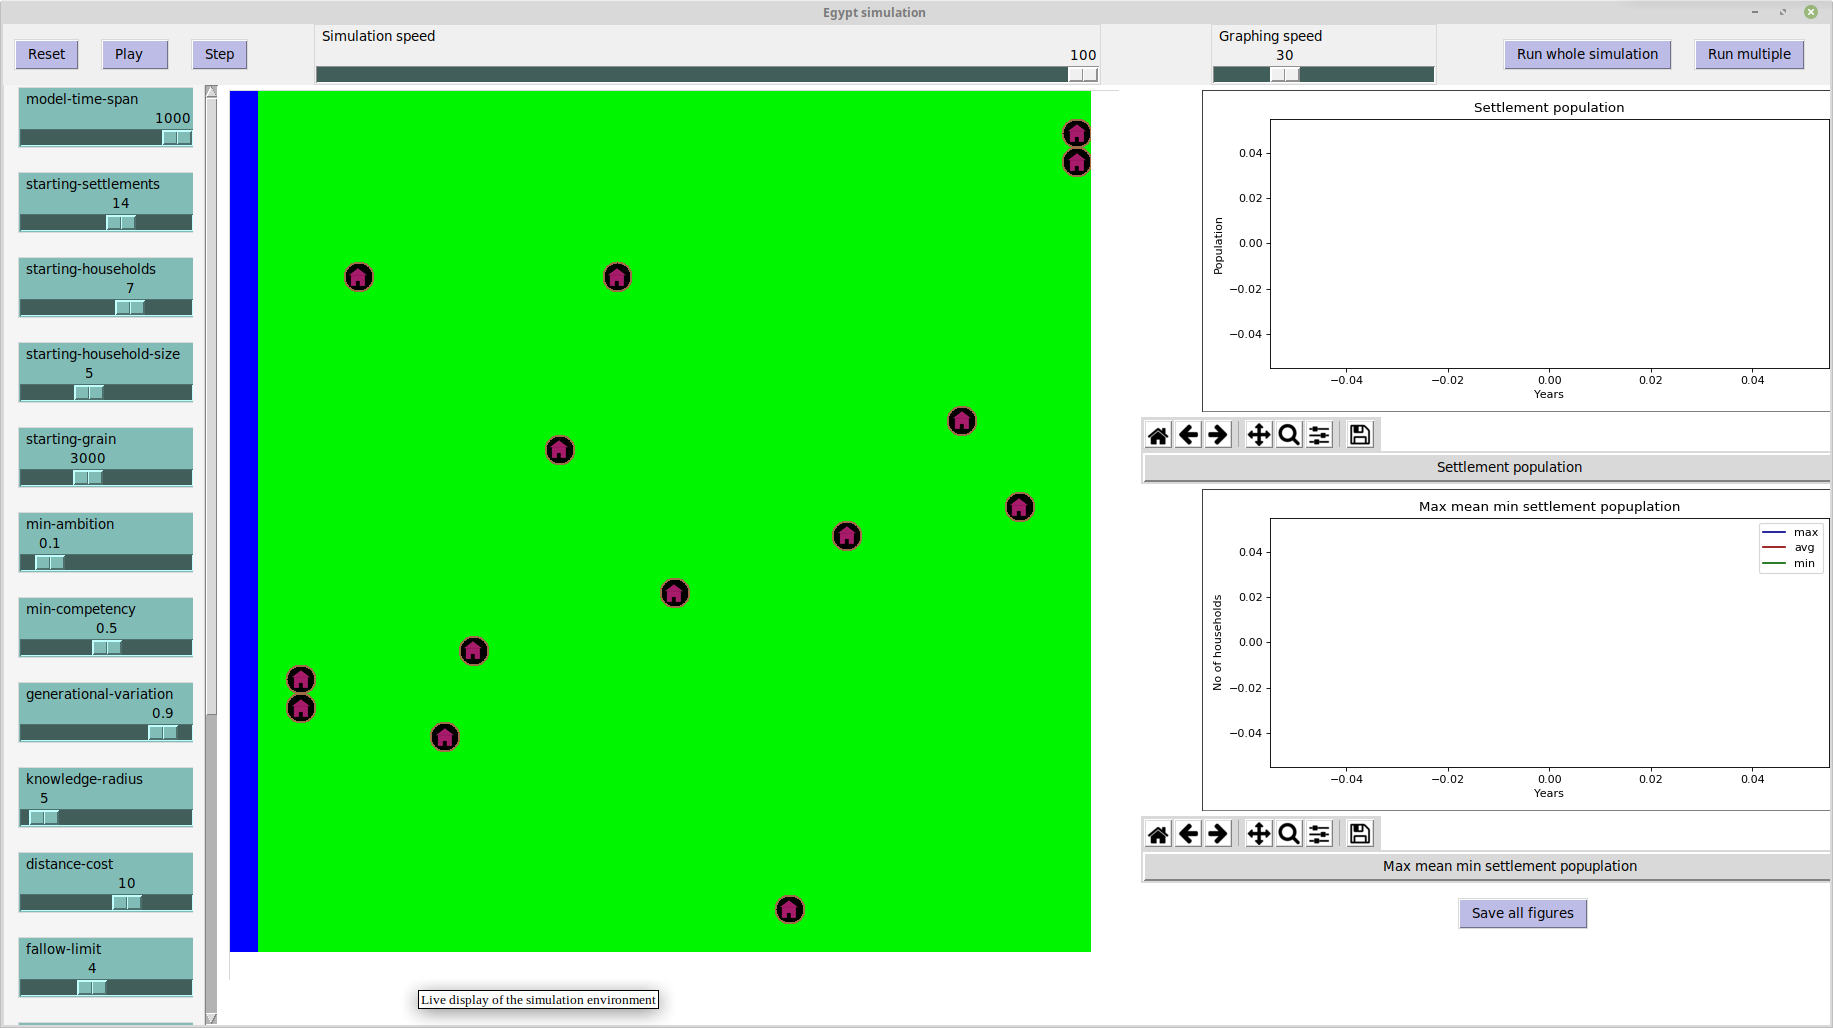
\includegraphics[width=15cm]{OnOpen}
		\caption{Screenshot of the application once opened, without any actions being performed.}
		\label{fig:OnOpen}
	\end{figure}
	
	\begin{figure}[!htb]
		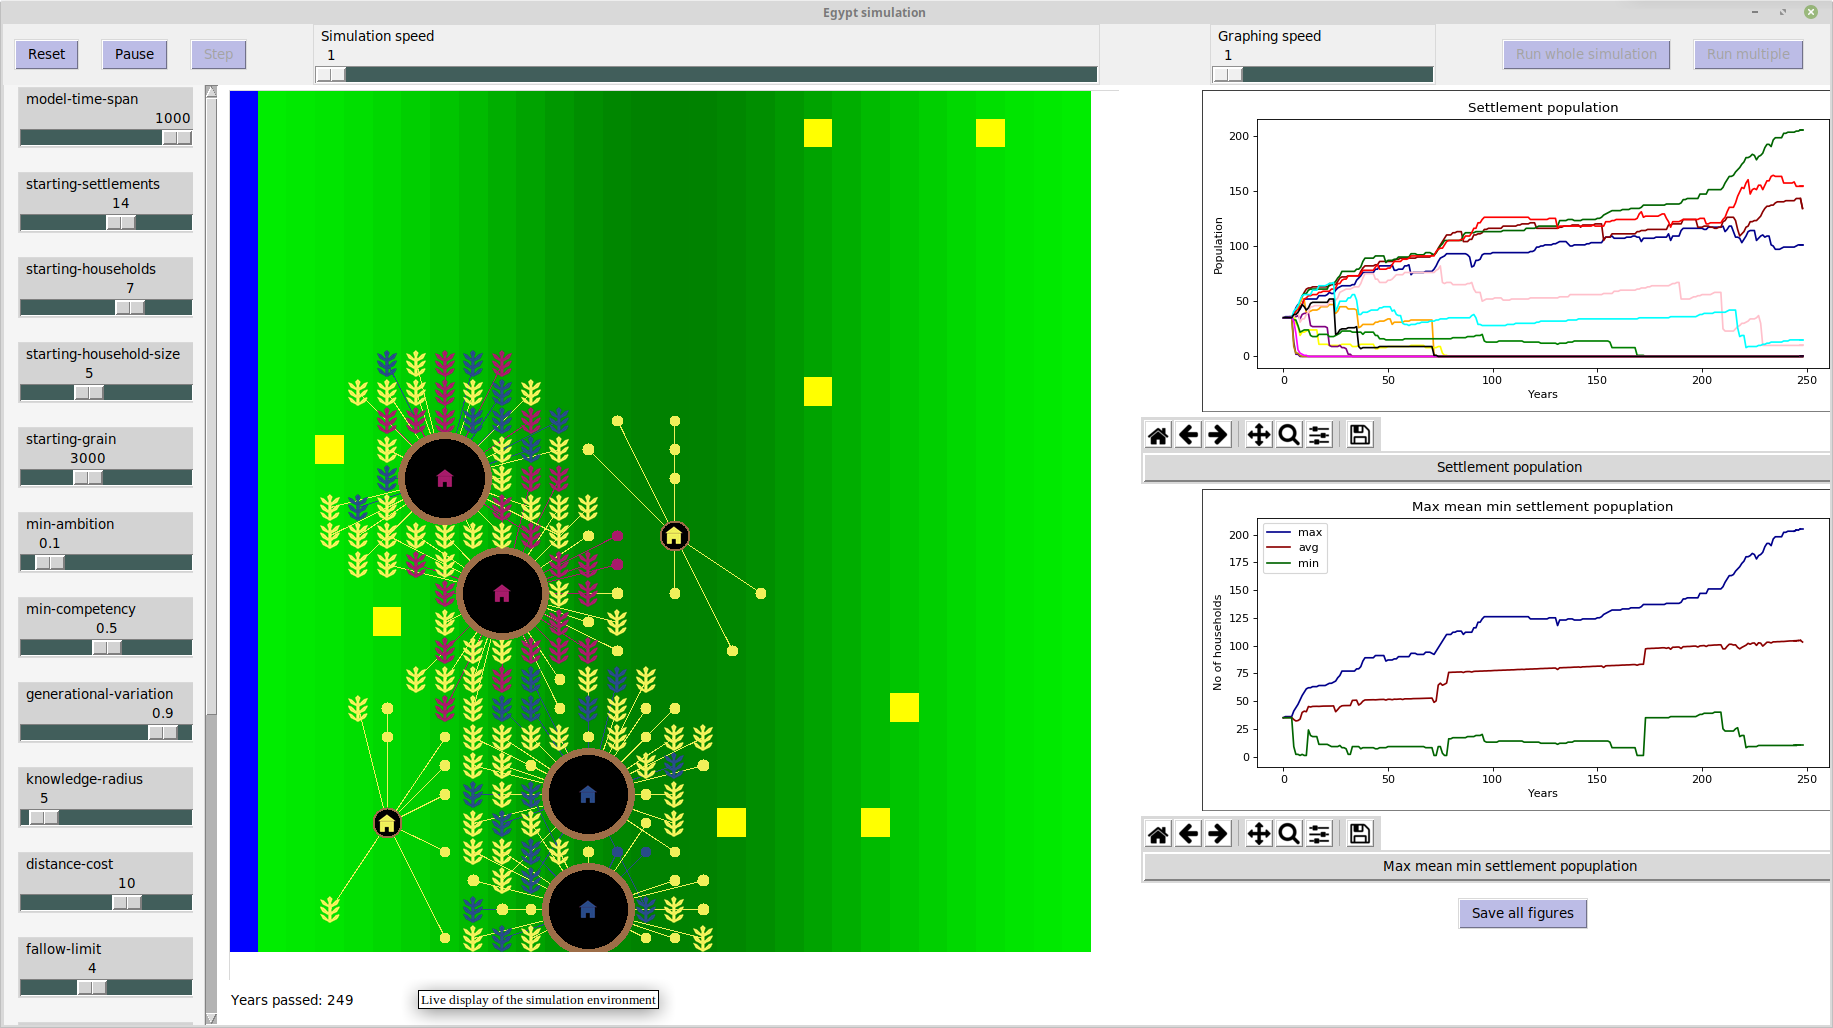
\includegraphics[width=15cm]{WhileRunning}
		\caption{Screenshot of the application once a run has begun, taken at a slow simulation speed to prevent screentearing during a screenshot.}
		\label{fig:WhileRunning}
	\end{figure}
	
	\begin{figure}[!htb]
		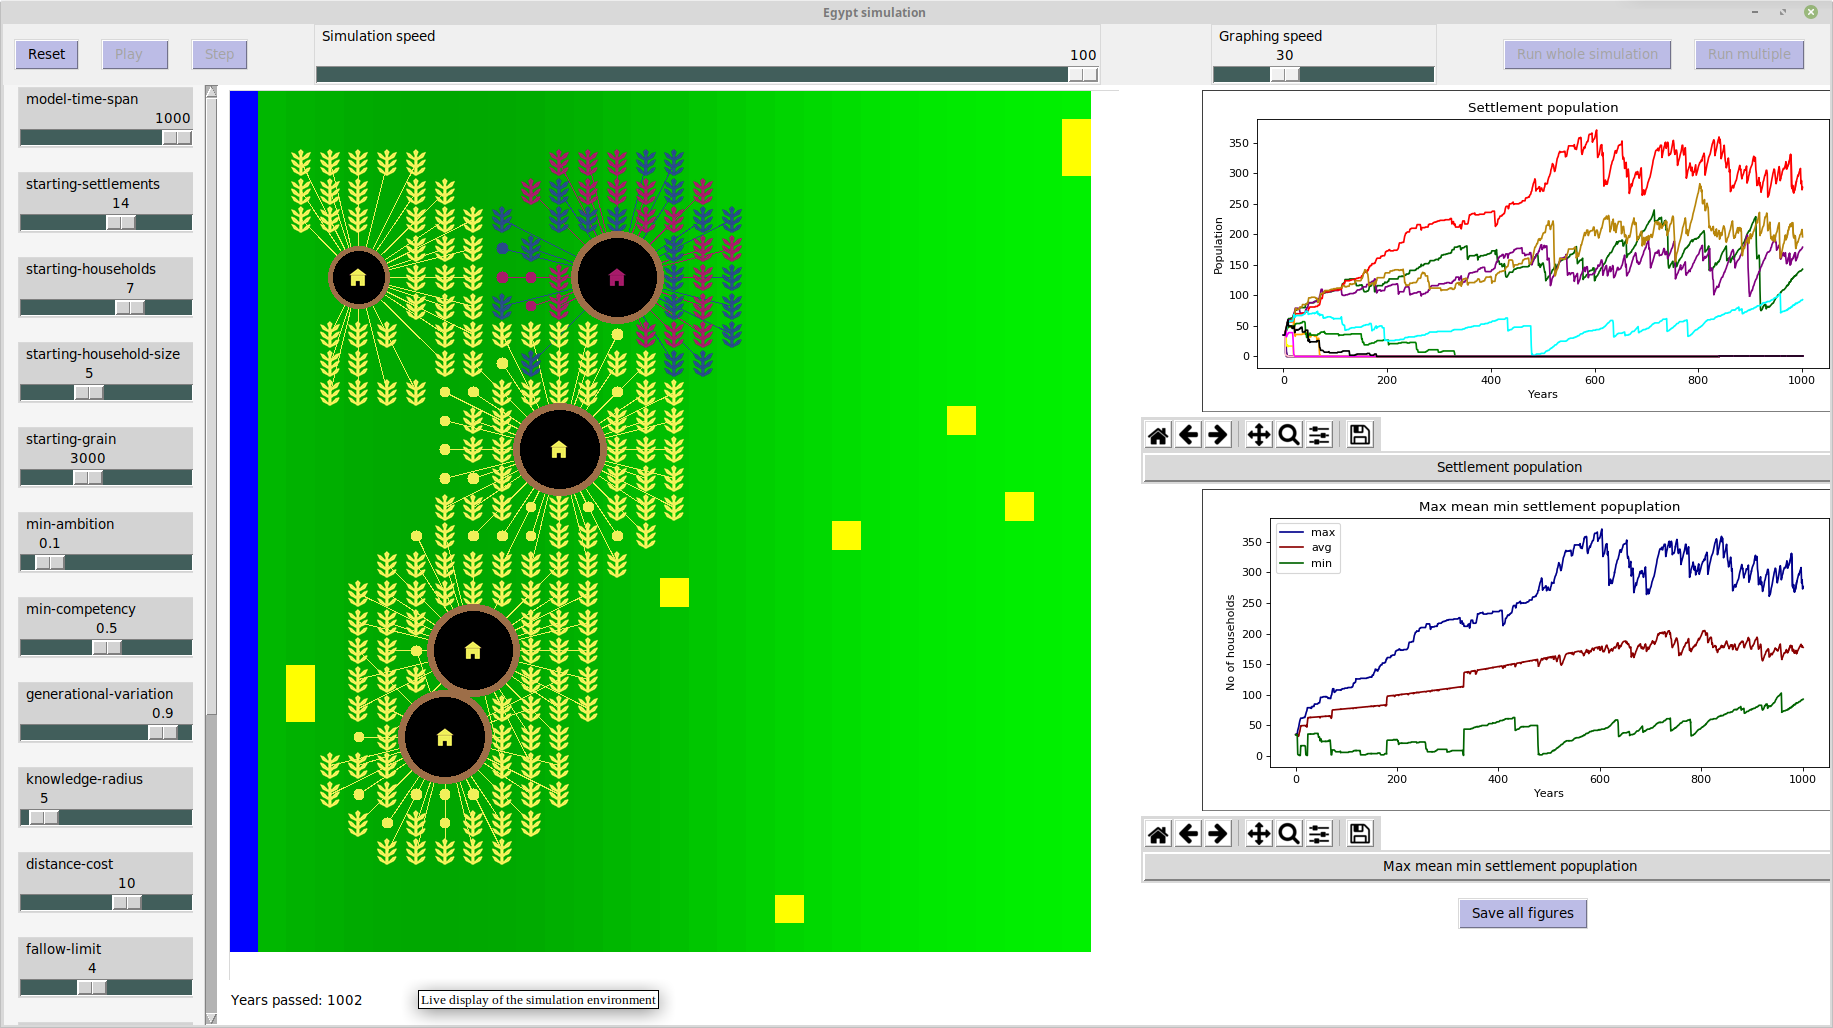
\includegraphics[width=15cm]{FinishedRunning}
		\caption{Screenshot of the application once a run has completed.}
		\label{fig:FinishedRunning}
	\end{figure}
	
	\begin{figure}[!htb]
		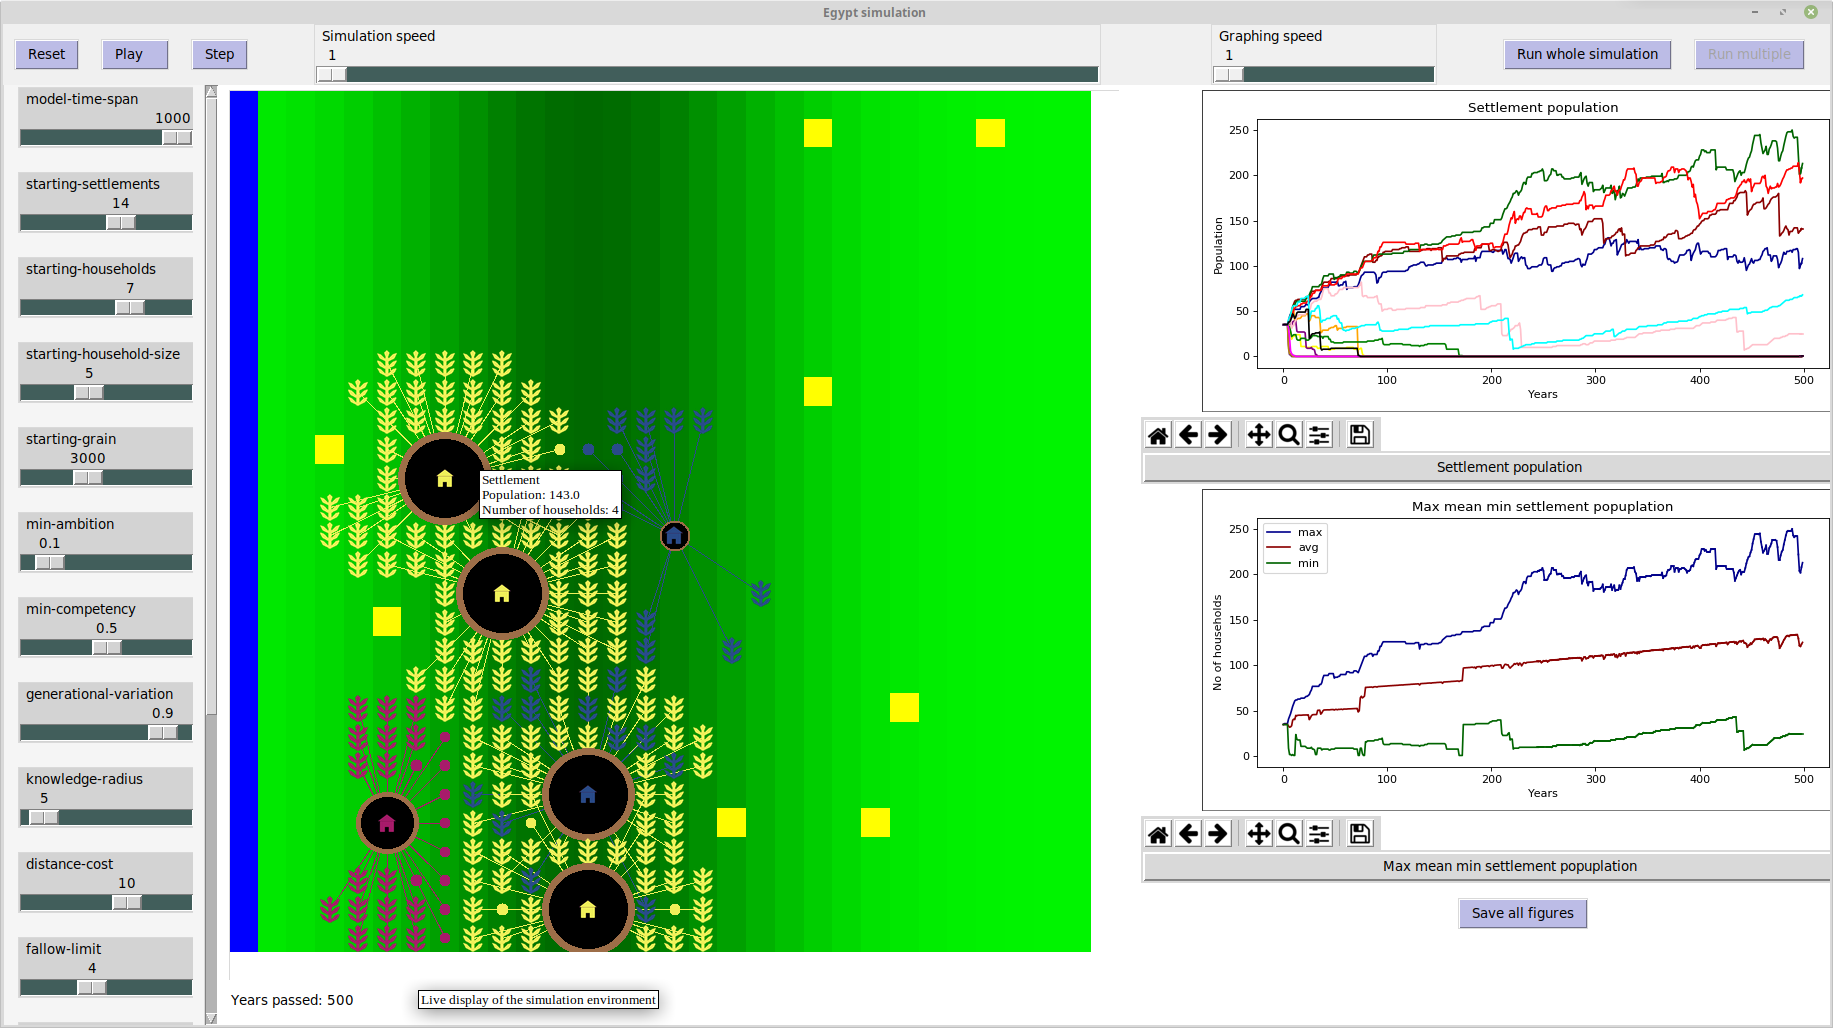
\includegraphics[width=15cm]{RightClickOnSettlement}
		\caption{Screenshot of the application during a run, with the simulation paused and the output of right clicking on a settlement shown.}
		\label{fig:ClickOnSettlement}
	\end{figure}
	
	\begin{figure}[!htb]
		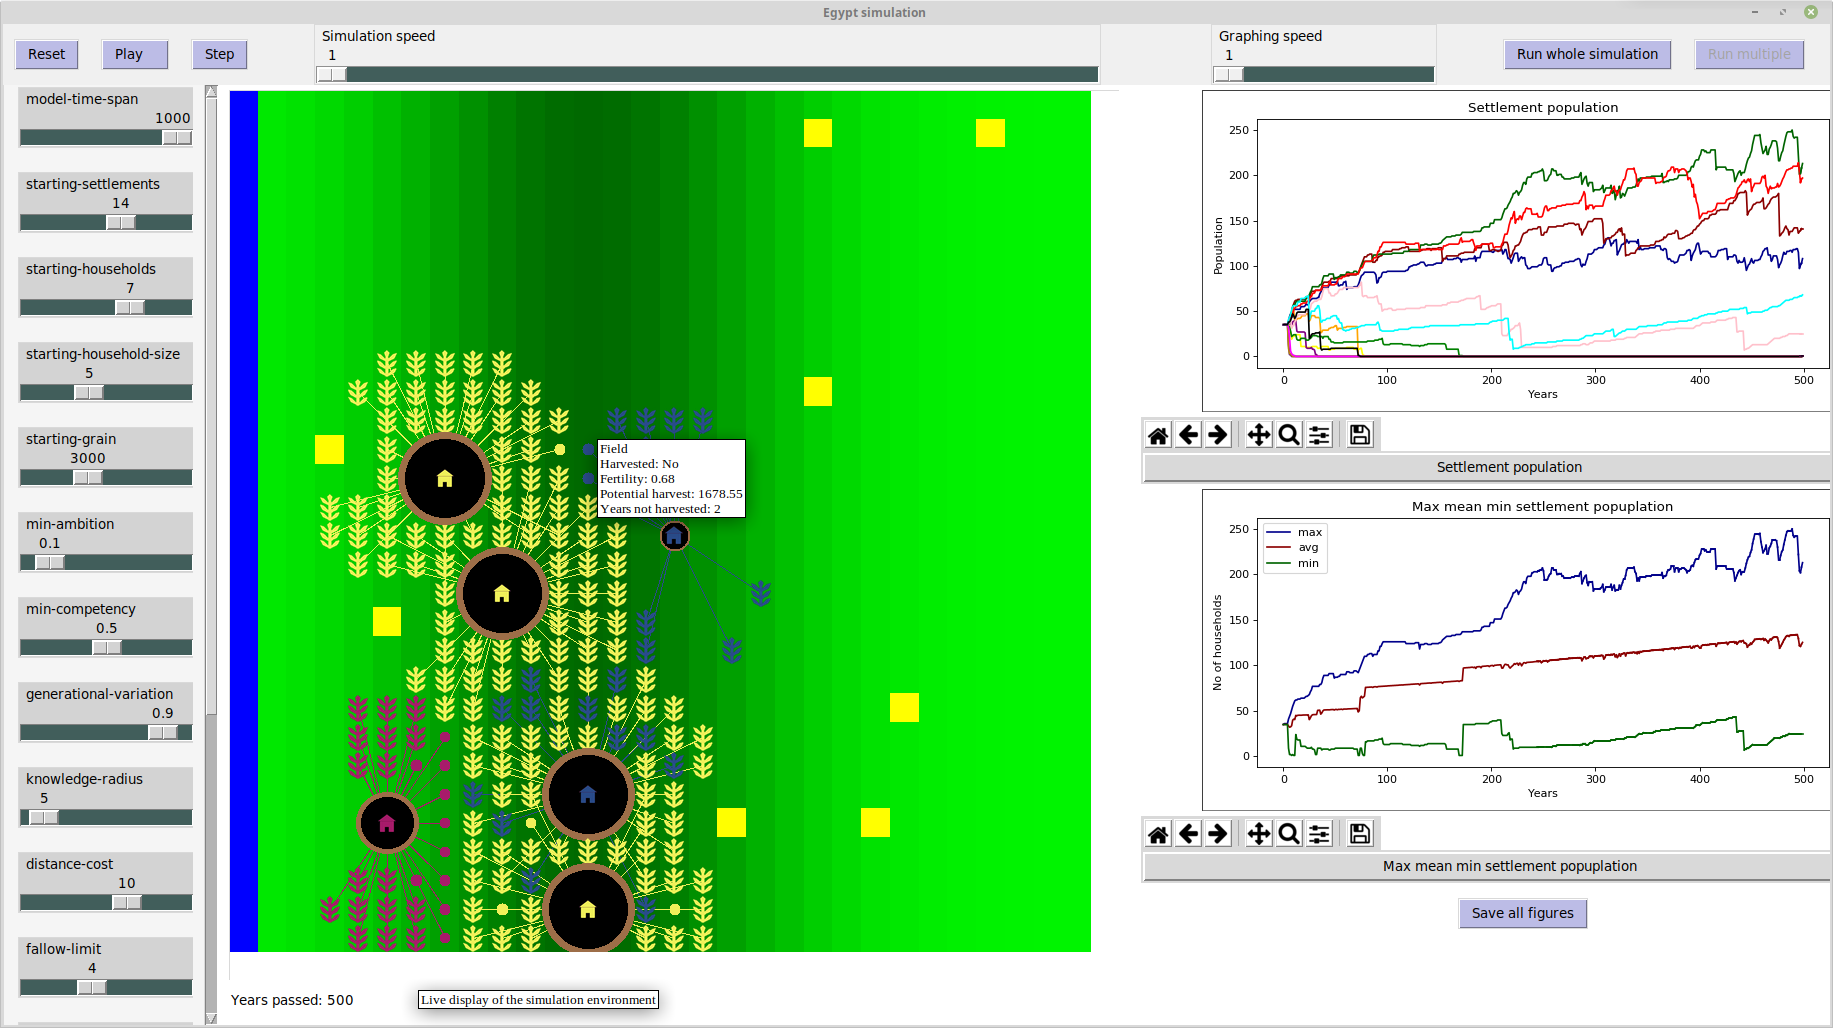
\includegraphics[width=15cm]{RightClickOnNotHarvestedField}
		\caption{Screenshot of the application during a run, with the simulation paused and the output of right clicking on an unharvested field shown.}
		\label{fig:ClickOnUnharvested}
	\end{figure}
	
	\begin{figure}[!htb]
		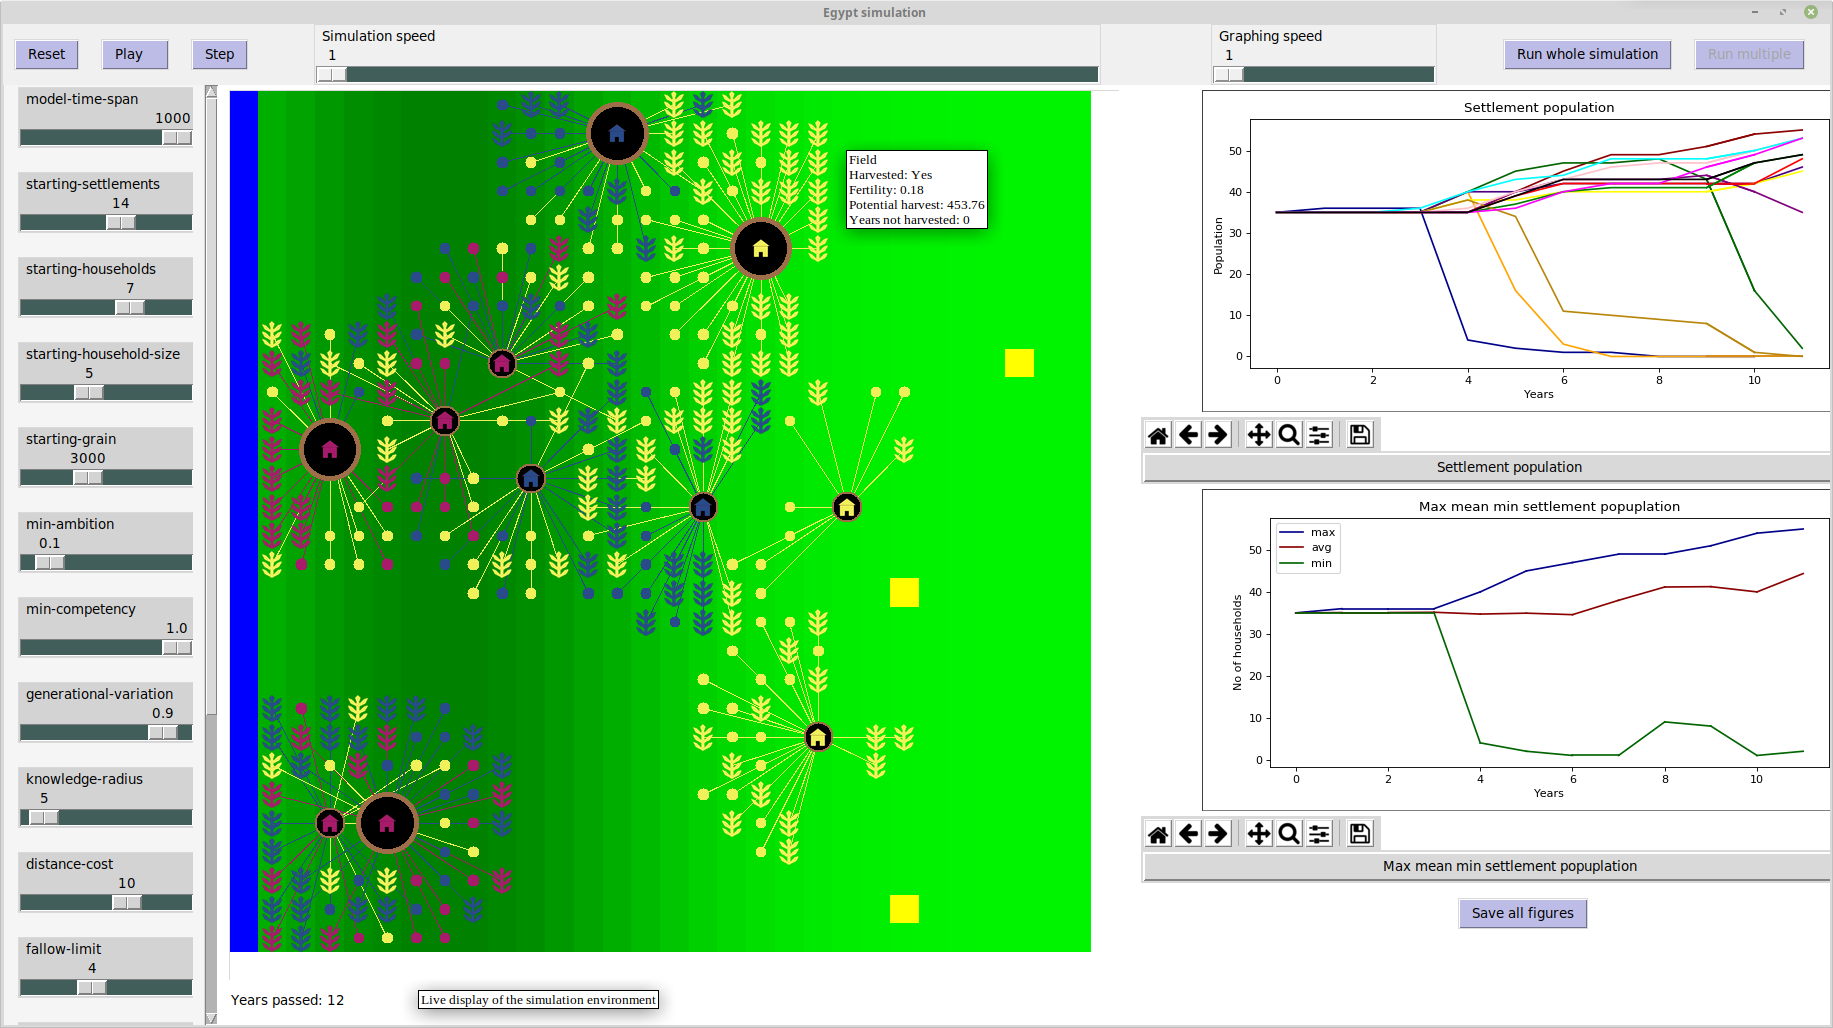
\includegraphics[width=15cm]{RightClickOnHarvestedField}
		\caption{Screenshot of the application during a run, with the simulation paused and the output of right clicking on a harvested field shown.}
		\label{fig:ClickOnHarvested}
	\end{figure}
	
	\begin{figure}[!htb]
		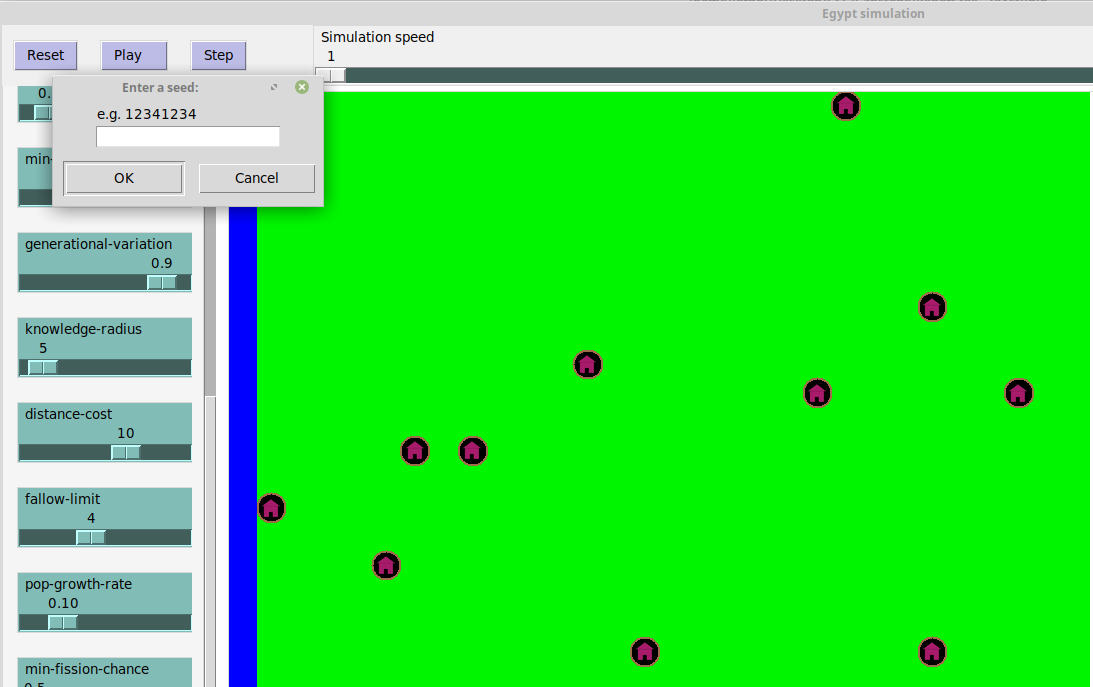
\includegraphics[width=15cm]{SeedEntry}
		\caption{Screenshot of the application showing how a manual seed is entered.}
		\label{fig:Seed Entry}
	\end{figure}
\end{document}